% !TEX program = xelatex
%% Requires compilation with XeLaTeX or LuaLaTeX
\documentclass[10pt,xcolor={table,dvipsnames},t]{beamer}
\usepackage{biblatex}
\usepackage{caption}
\setbeamertemplate{caption}[numbered]
\addbibresource{reference.bib}
\usepackage{hyperref}
\hypersetup{ 
pdfpagemode=FullScreen,  
colorlinks=true,linkcolor=blue}
\usepackage{enumerate}
\usepackage{algorithm}
\usepackage{algpseudocode}
\usepackage{listings}
\usepackage{xcolor}
\usepackage{graphicx}

\graphicspath{{./img/}}

\definecolor{codegreen}{rgb}{0,0.6,0}
\definecolor{codegray}{rgb}{0.5,0.5,0.5}
\definecolor{codepurple}{rgb}{0.58,0,0.82}
\definecolor{backcolour}{rgb}{0.95,0.95,0.92}

\lstdefinestyle{mystyle}{
    backgroundcolor=\color{backcolour},   
    commentstyle=\color{codegreen},
    keywordstyle=\color{magenta},
    numberstyle=\tiny\color{codegray},
    stringstyle=\color{codepurple},
    basicstyle=\ttfamily\footnotesize,
    breakatwhitespace=false,         
    breaklines=true,                 
    captionpos=b,                    
    keepspaces=true,                 
    numbers=left,                    
    numbersep=5pt,                  
    showspaces=false,                
    showstringspaces=false,
    showtabs=false,                  
    tabsize=2
}

\lstset{style=mystyle}

% Flow chart config
\usepackage{tikz}
\usetikzlibrary{calc,trees,positioning,arrows,fit,shapes,calc,tikzmark,matrix}
\usepackage{eso-pic}
\usetikzlibrary{shapes.geometric, arrows}
\tikzstyle{startstop} = [rectangle, rounded corners, minimum width=3cm, minimum height=1cm,text centered, draw=black, fill=red!30]
\tikzstyle{io} = [trapezium, trapezium left angle=70, trapezium right angle=110, minimum width=3cm, minimum height=1cm, text centered, draw=black, fill=blue!30]
\tikzstyle{process} = [rectangle, minimum width=3cm, minimum height=1cm, text centered, draw=black, fill=orange!30]
\tikzstyle{decision} = [diamond, minimum width=3cm, minimum height=1cm, text centered, draw=black, fill=green!30]
\tikzstyle{arrow} = [thick,->,>=stealth]

\usetheme{UCBerkeley}

\title[Your Short Title]{STMC Coding Team Training}
\subtitle{Lesson 9: HKOI question training}
\author{Tsai Yun Chen}
%\institute{}
\date{\today}

\begin{document}

\begin{frame}
  \titlepage
\end{frame}

% Uncomment these lines for an automatically generated outline.
%\begin{frame}{Outline}
%  \tableofcontents
%\end{frame}

\section{Class Goal}

\begin{frame}{Goal today}
Today we will practice several questions on the platform of HKOI.
\begin{itemize}
  \item 01033 Simple Arithmetic
  \item 01015 Parenthesis Balance
  \item 01077 Course Registration
  \item 01017 Car Sorter
  \item Challenge: M1313 Bookstack
\end{itemize}
\end{frame}

\begin{frame}{Simple Arithmetic}
  \begin{figure}[h!]
    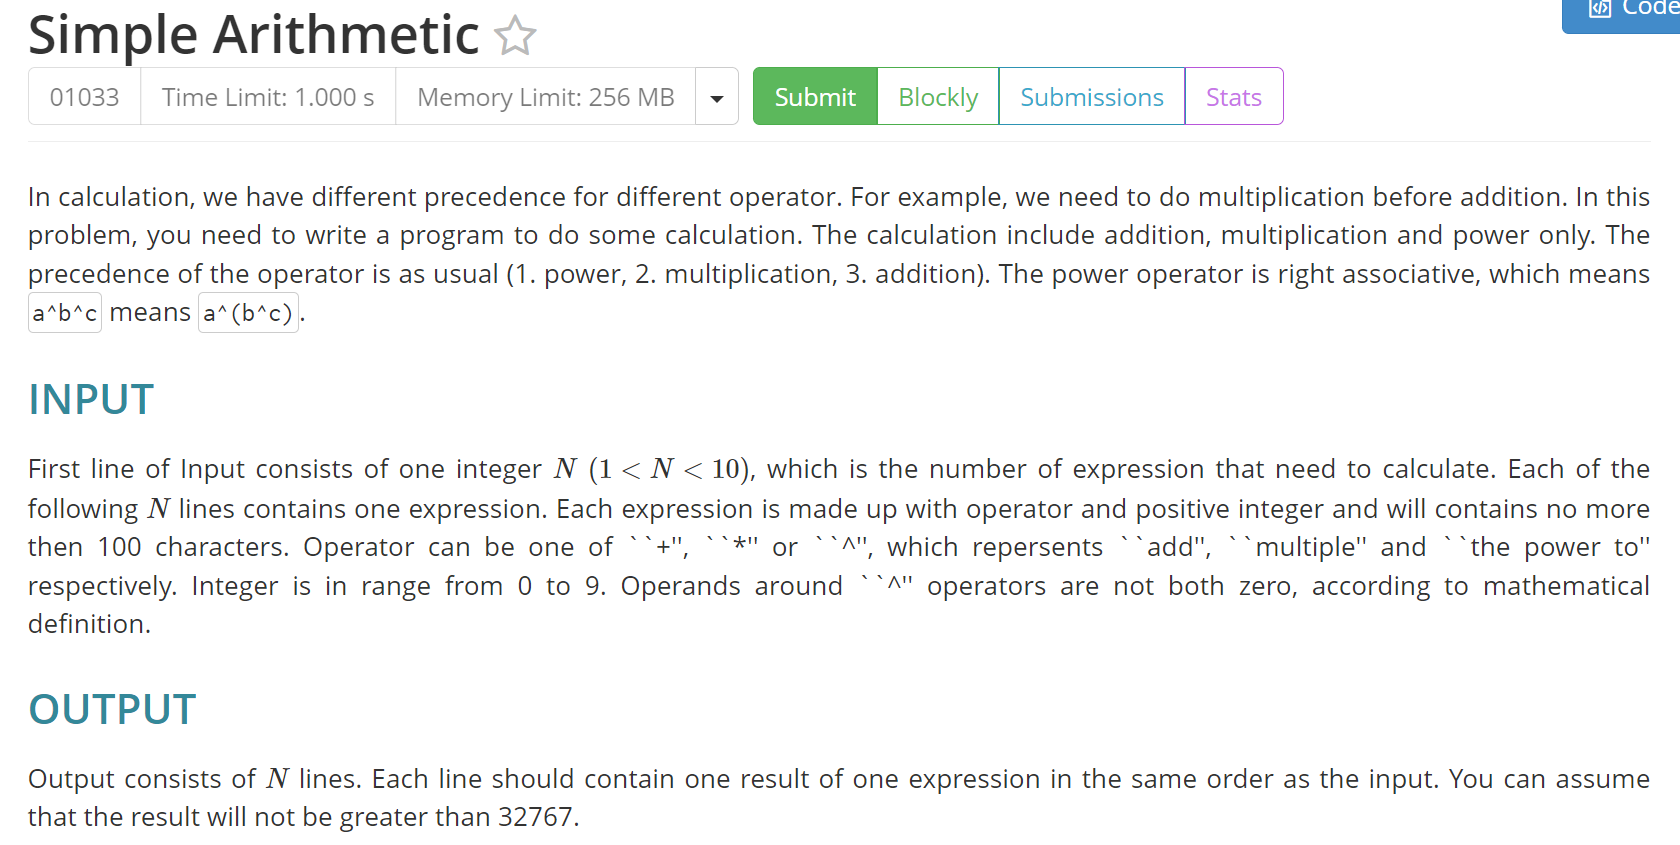
\includegraphics[width=0.7\textwidth]{Q1.png}
    \caption{Simple Arithmetic(\href{https://judge.hkoi.org/task/01033}{Source})}
  \end{figure}
\end{frame}

\begin{frame}{Hint}
  \begin{itemize}
    \item Recall the topic we convered last lecture
    \item slightly modify the code to obtain the solution
  \end{itemize}
\end{frame}

\begin{frame}{Parenthesis Balance}
  \begin{figure}[h!]
    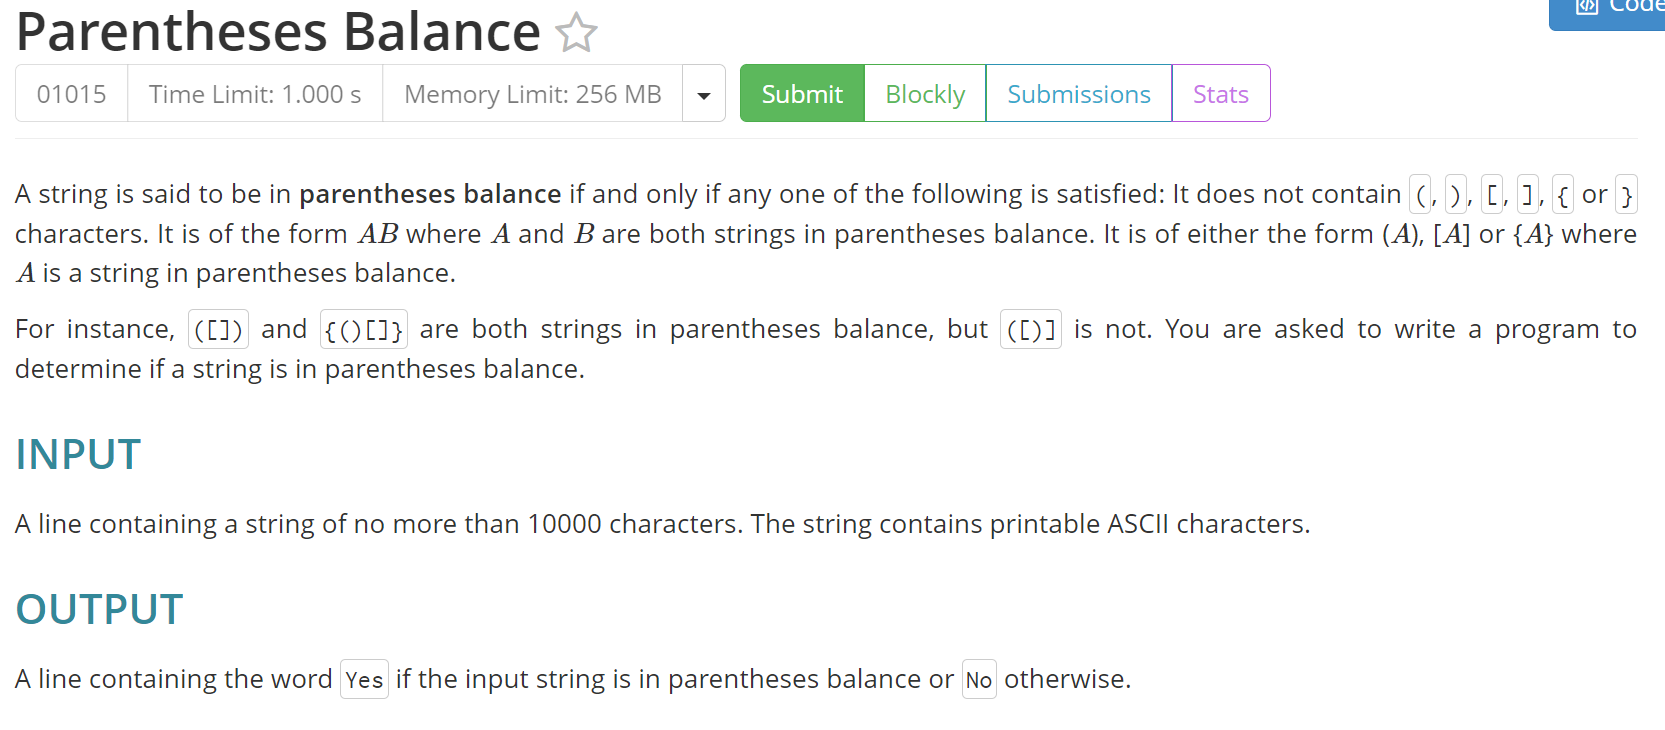
\includegraphics[width=0.7\textwidth]{Q2.png}
    \caption{Parenthesis Balance(\href{https://judge.hkoi.org/task/01015}{Source})}
  \end{figure}
\end{frame}

\begin{frame}{Hint}
  \begin{itemize}
    \item Stack is the key to this problem
    \item imagine walking along the string of parenthesis, if you met a close parenthesis
    \begin{itemize}
      \item )
      \item ]
      \item \}
    \end{itemize}
    \item then what you should you expect when you look back?
  \end{itemize}
\end{frame}

\begin{frame}{Course Registration}
  \begin{figure}[h!]
    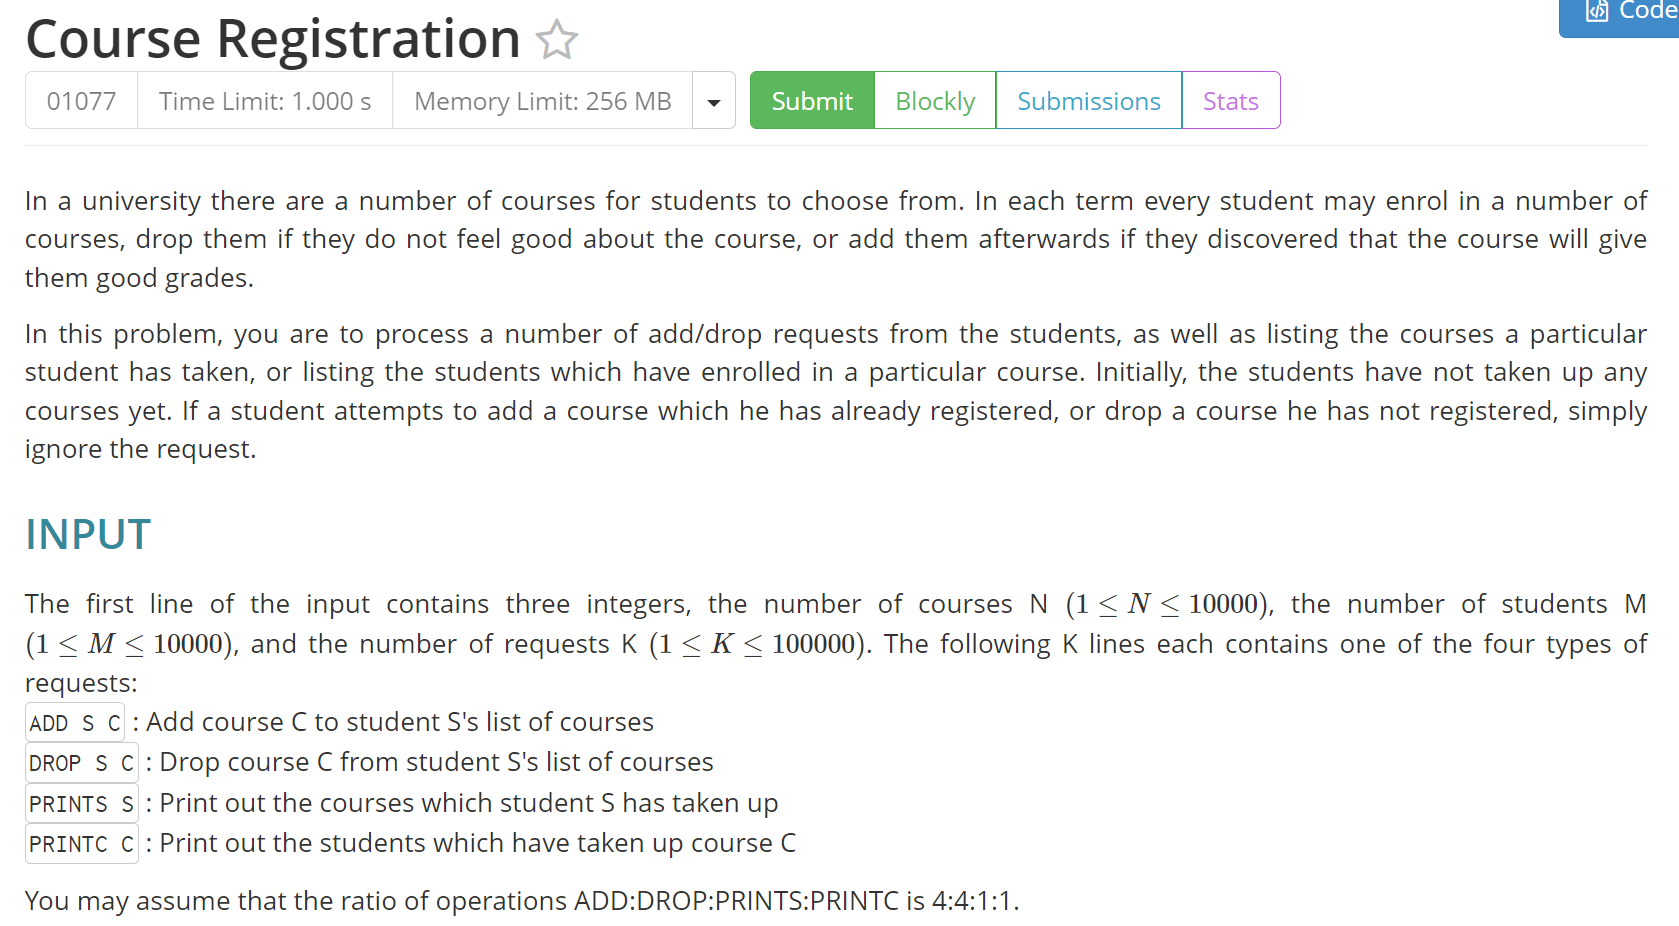
\includegraphics[width=0.7\textwidth]{Q3.png}
    \caption{Course Registration(\href{https://judge.hkoi.org/task/01077}{Source})}
  \end{figure}
\end{frame}

\begin{frame}{Hint}
  \begin{itemize}
    \item Question suggested the add and drop query is a lot more
    \item so update should be efficient, but searching need not
    \item the number of data is fixed (this is important!)
    \item we don't need stack or queue here
  \end{itemize}
\end{frame}

\begin{frame}{Car Sorter}
  \begin{figure}[h!]
    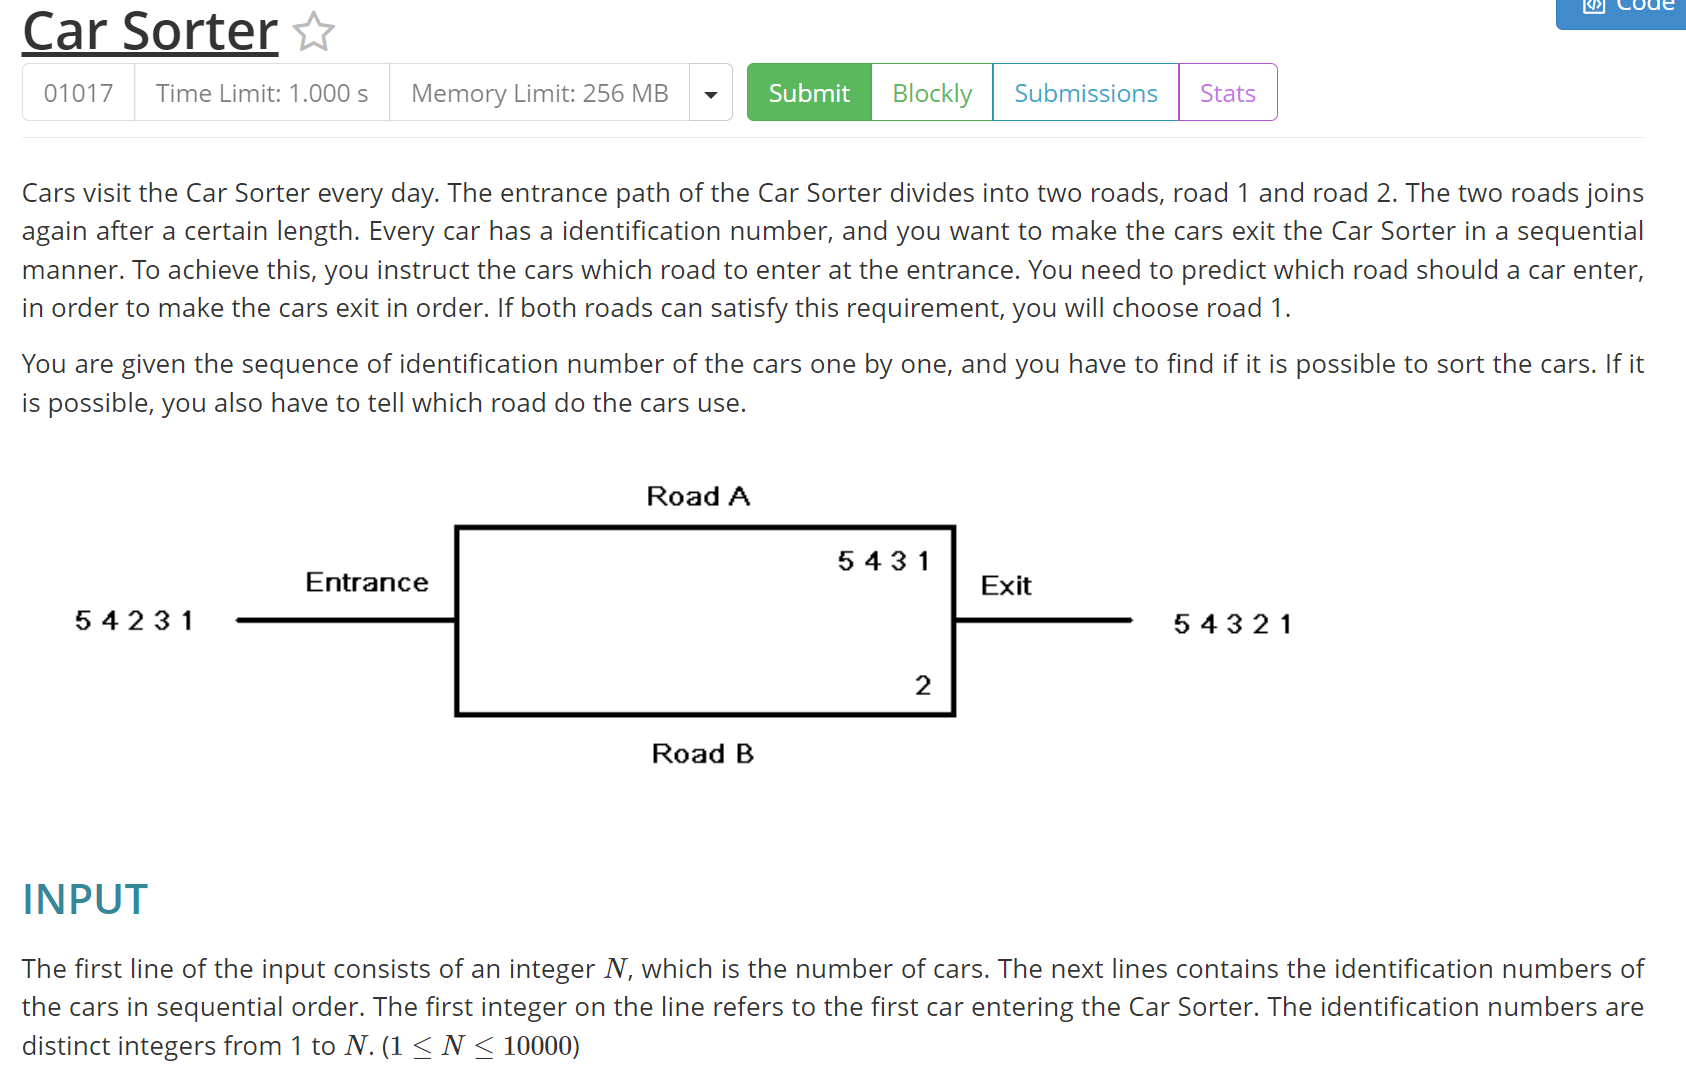
\includegraphics[width=0.7\textwidth]{Q4.png}
    \caption{Car Sorter(\href{https://judge.hkoi.org/task/01017}{Source})}
  \end{figure}
\end{frame}

\begin{frame}{Hint}
  \begin{itemize}
    \item consider maintaining two queues
    \item think carefully which queue you should add the car to
  \end{itemize}
\end{frame}

\begin{frame}{Bookstack}
  \begin{figure}[h!]
    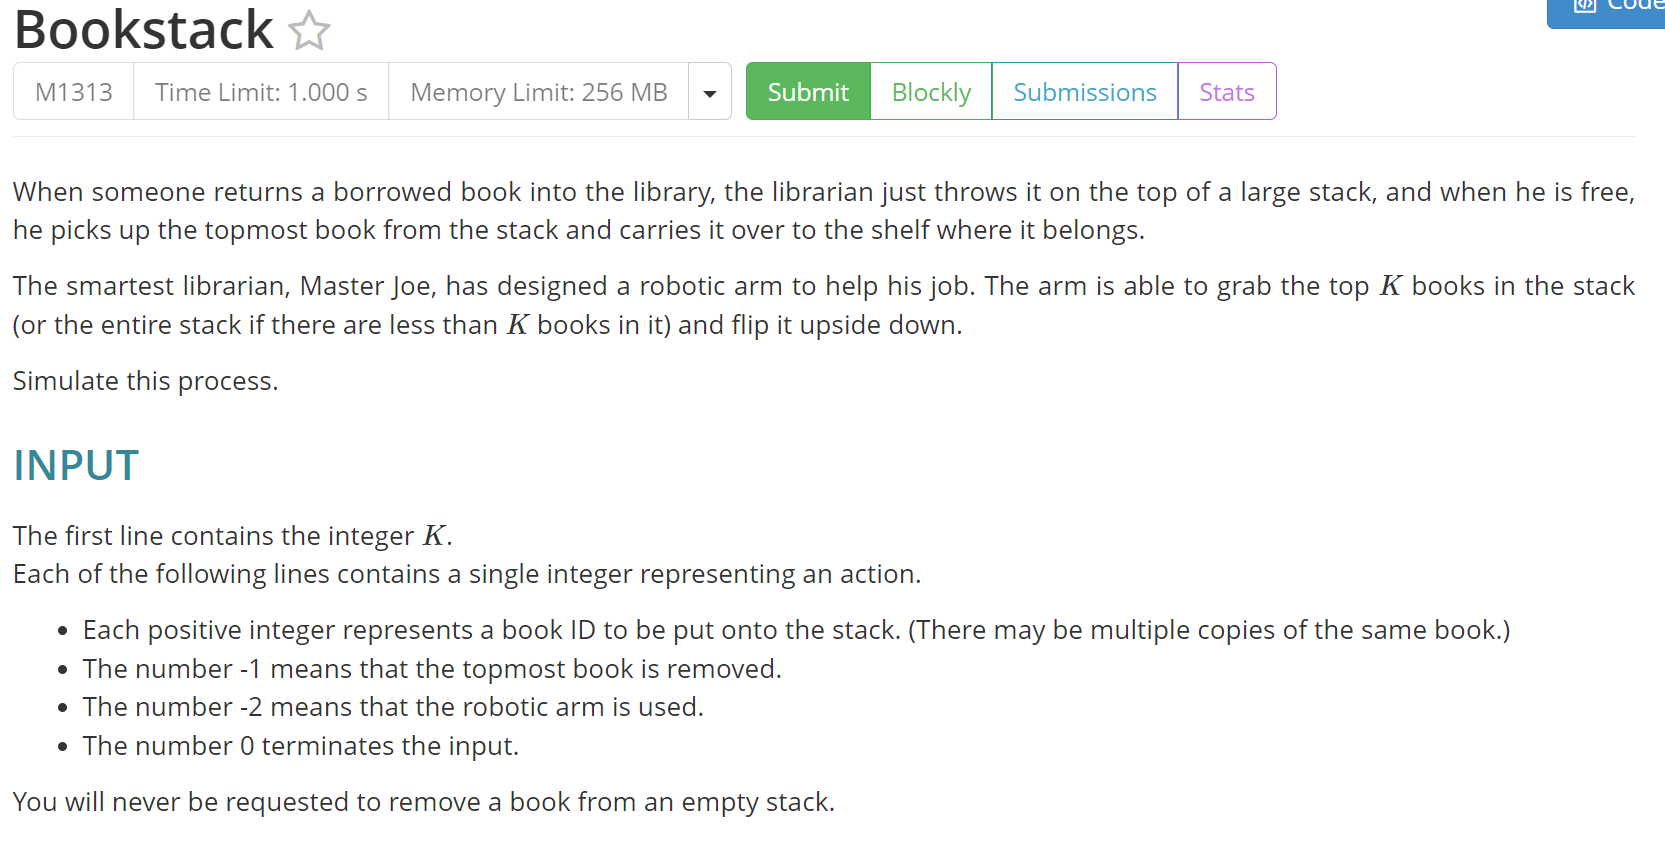
\includegraphics[width=0.7\textwidth]{Q5.png}
    \caption{Bookstack(\href{https://judge.hkoi.org/task/M1313}{Source})}
  \end{figure}
\end{frame}

\begin{frame}{Hint}
  \begin{itemize}
    \item This is a challenge one
    \item as name suggested you need to use stack
    \item the number K is important
    \item a big hint: conasider an array of stack
  \end{itemize}
\end{frame}
\end{document}
